\section{Social Media - III Lecture}

\subsection{Social CRM Technology}\label{social-crm-technology}

\subsubsection{Definition and Tools}\label{definition-and-tools}

\begin{figure}[!h]
    \centering
    \includegraphics[page=24, trim = 1.5cm 5cm 1.5cm 4cm, clip, width=\textwidth]{images/04 - Social_Media.pdf}
\end{figure}

Social CRM technology refers to the tools and systems that companies can
utilize to effectively manage their presence on social media platforms.
It is an extension of traditional customer relationship management (CRM)
that incorporates social functionalities. These tools are specifically
designed to handle the unique challenges and opportunities presented by
social media.

Unlike traditional CRM systems, social CRM tools are tailored to manage
interactions and engagements on social media platforms. They enable
companies to monitor and analyze social media conversations, track
customer sentiment, and respond to customer inquiries and feedback in a
timely manner. These tools also provide valuable insights into customer
behavior and preferences, allowing companies to personalize their
interactions and deliver targeted marketing campaigns.

Some popular social CRM tools include social listening platforms, social
media management systems, and social analytics software. These tools
help companies streamline their social media management processes,
improve customer engagement, and enhance their overall social media
presence.

In summary, social CRM technology offers companies the means to
effectively manage their social media presence and engage with customers
on these platforms. It complements traditional CRM systems by
incorporating social functionalities and providing tools specifically
designed for social media management.

\subsubsection{Community Support and
    Management}\label{community-support-and-management}

In the realm of social CRM, large companies often begin by supporting a
private label community. This can take the form of a Facebook fan page
or a community built around a mobile app. The next step is monitoring.
This involves listening to and surveying both private label social
networks and independent social networks to expand the reach of
listening to potential clients. Once the community is established,
companies can use various tools to activate the community, encourage
content sharing, foster a sense of community, and ultimately obtain
product reviews and facilitate online sales. However, managing these
interactions can be challenging, which is where social CRM comes in to
assist.

\subsubsection{Functionalities of Social
    CRM}\label{functionalities-of-social-crm}

\begin{figure}[!h]
    \centering
    \includegraphics[page=25, trim = 0cm 3.5cm 5cm 0.5cm, clip, width=\textwidth]{images/04 - Social_Media.pdf}
\end{figure}

\paragraph{User Functionalities}\label{user-functionalities}
Social CRM technology offers a range of user functionalities that are
primarily used by a company's internal users, such as marketing
employees. These functionalities include discussion forums, where
marketing employees can act as moderators, message boards, polls, and
voting. These features allow companies to engage with their client base
and gather feedback on preferences, such as product changes or color
options. Additionally, social CRM provides functionalities for reviews,
ratings, chat management (including the ability to save conversations),
blog management, and wiki management. These various functionalities
contribute to the comprehensive capabilities of social CRM technology.

\begin{figure}[!h]
    \centering
    \includegraphics[page=26, trim = 0cm 5.5cm 5cm 0.5cm, clip, width=\textwidth]{images/04 - Social_Media.pdf}
\end{figure}

\paragraph{Administrative
    Functionalities}\label{administrative-functionalities}
In addition to the various functionalities of social CRM, there are also
several administrative functionalities available. These include
moderation, reputation management, dashboards, reports, events
management, privacy management, video management, and outbound campaign
functionalities. It's important to note that these administrative
functionalities are primarily intended for internal use within the
organization, specifically for administrative purposes. On the other
hand, when we refer to the users of polls and voting as internal
employees, it means that they have the ability to set up these
functionalities for external users to utilize.

In addition to traditional CRM, social CRM also offers outbound campaign
functionalities. Just like in traditional CRM, campaign management is a
key feature of social CRM. Companies frequently manage campaigns on
social media platforms. One of the benefits of using social CRM is the
ability to manage multiple social media platforms from one integrated
dashboard. For example, companies can create content, compose a post,
and then publish it on multiple social media platforms simultaneously.

\subsection{Social CRM vs.~Listening
    Platforms}\label{social-crm-vs.-listening-platforms}

\begin{figure}[!h]
    \centering
    \includegraphics[page=27, trim = 1.5cm 6cm 2.5cm 0.5cm, clip, width=\textwidth]{images/04 - Social_Media.pdf}
\end{figure}

\subsubsection{Integration and
    Differences}\label{integration-and-differences}

In the field of marketing, there are various tools that marketing
employees need to use. For example, when managing campaigns, they may
use social media platforms like Facebook, blogs, private label social
networks, forums, and more. If these platforms are owned and managed by
the company, they can utilize social CRM. However, when it comes to
budget administration and reaching potential clients on social media to
drive traffic to the company's website or encourage app downloads, they
need to use the dashboards and applications provided by different global
social media platforms such as Facebook and Google Ads.

One challenge with CRM is that the management of outbound campaigns on
the web and social media lacks integration. Companies are still waiting
for a tool that can integrate the management of all these channels into
one platform. It's important to note the distinction between social CRM
and listening platforms. While social CRM may or may not integrate a
listening platform, it can perform surveys and interact directly with
clients or potential clients. However, it may not be able to collect
spontaneous information from social media and provide a summary of the
main drivers of conversation or the sentiment surrounding different
aspects of their products. Listening is a crucial first step, and many
companies use a separate tool for this purpose, different from social
CRM.

\paragraph{Examples of Listening
    Platforms}\label{examples-of-listening-platforms}

An example of a listening platform is Nielsen
Buzzmetrics. This platform specializes in collecting information from
social media related to a specific brand or set of keywords. It then
generates a comprehensive report based on this data.

\subsubsection{Evolution of the Market}\label{evolution-of-the-market}

\begin{figure}[!h]
    \centering
    \includegraphics[page=28, trim = 1.5cm 1.5cm 2.5cm 3.5cm, clip, width=\textwidth]{images/04 - Social_Media.pdf}
\end{figure}

Many companies choose not to handle social media monitoring in-house and
instead opt to hire consulting firms. These firms utilize multiple
listening platforms to gather data from various sources and provide an
integrated view of a company's reputation on social media. The market
for social media intelligence has evolved over time, progressing from
simple text analytics to web intelligence and then to social media
intelligence in 2005. After 2010, the market further expanded to include
multimedia intelligence. Since 2014, traditional software vendors have
begun integrating social media intelligence into their tools. However,
it is worth noting that the best tools for social CRM are often separate
from traditional CRM systems. In many cases, companies use a different
tool for social CRM compared to their traditional CRM tool.

\subsection{Data Sources and Analytics}\label{data-sources-and-analytics}

\subsubsection{Challenges with Data
    Sources}\label{challenges-with-data-sources}

\begin{figure}[!h]
    \centering
    \includegraphics[page=30, trim = 1cm 6.5cm 2cm 3.5cm, clip, width=\textwidth]{images/04 - Social_Media.pdf}
\end{figure}

When it comes to data sources, it's important to consider the vastness
of the web. While tools for listening claim to survey the web in
general, they may not effectively distinguish between institutional
websites and social media platforms. These two types of sources are
fundamentally different. Institutional web refers to official news
sources and company websites, while social media includes platforms like
Facebook, Instagram, and Twitter.

It's crucial to recognize this distinction because the institutional web
does not necessarily represent the potential client base. Therefore,
it's necessary to survey and understand these sources separately, as
well as manage them independently.

One common issue with listening tools is that they can be misleading. In
some cases, these tools may not provide an accurate list of sources,
focusing only on social media and excluding the institutional web. They
may also claim to survey a wide range of sources, such as blogs, forums,
news, and social media in a generic manner. However, this generic
approach can lead to varying indications of a company's reputation when
different tools are used. This inconsistency is a pervasive problem in
these types of applications.

\subsubsection{Sentiment Analysis and
    Precision}\label{sentiment-analysis-and-precision}

\begin{figure}[!h]
    \centering
    \includegraphics[page=31, trim = 1.5cm 1.8cm 2.5cm 0.5cm, clip, width=\textwidth]{images/04 - Social_Media.pdf}
\end{figure}

In addition to lacking insights, these companies also apply very little
intelligence to the information they receive. For instance, they fail to
provide data on the precision of their tools. To illustrate this point,
let's consider the example of sentiment analysis, specifically regarding
people's opinions on the health impact of Nutella, one of Ferrero's brands.
To accurately analyze sentiment, it is crucial to correctly identify the
brand, categorize the posts based on topic, and assess whether people
are discussing health issues. For example, if a client says, ``I wasn't
feeling good yesterday, but a spoonful of Nutella cheered me up,'' how
should this post be interpreted? Well, it conveys a positive sentiment
towards Nutella and does not discuss health concerns. This is not the
desired outcome.

Typically, companies provide separate precision results for brand
identification, categorization, and sentiment analysis. However, when
these three dimensions need to be executed consecutively and accurately,
the overall precision is typically the product of the individual
precisions. This means that even if each dimension has a precision of
0.7 (70\%), the overall precision becomes like tossing a coin, resulting
in a 50\% precision for sentiment analysis. In other words, the
information obtained, especially regarding sentiment analysis, may not
be accurate.

When companies fail to provide accurate data, it poses a problem.
Reports without accuracy information may still be useful as they provide
a general idea of the topics being discussed. However, sentiment
analysis has not yet produced a standout application that justifies
investing in the quality of results. The overall quality of these
analyses tends to be poor.

\subsection{Future of Social Media
    Tools}\label{future-of-social-media-tools}

\subsubsection{Real-Time Services and
    Geolocation}\label{real-time-services-and-geolocation}

\begin{figure}[!h]
    \centering
    \includegraphics[page=32, trim = 1cm 4.5cm 1cm 3cm, clip, width=\textwidth]{images/04 - Social_Media.pdf}
\end{figure}

Another issue is the lack of real-time services offered by these
companies. Many sources do not guarantee real-time updates and often
have delays. In the context of social media, real-time should truly mean
real-time. A 20-minute delay on social media is unacceptable, as the
hype surrounding a topic can die down within half an hour. On the other
hand, a 50-minute delay on news platforms like GDELT project by Google is
acceptable, as news and institutional websites do not have the same
dynamic nature as social media.

\subsubsection{Industry-Specific
    Solutions}\label{industry-specific-solutions}

\begin{figure}[!h]
    \centering
    \includegraphics[page=33, trim = 1cm 8cm 1cm 3.5cm, clip, width=\textwidth]{images/04 - Social_Media.pdf}
\end{figure}

In order to make informed marketing decisions, it is crucial to have
access to high-quality tools and information from reliable suppliers.
This requires us to be knowledgeable and discerning in the market.
Unfortunately, there are only a few tools available that provide
geolocation information, which can be valuable for marketing purposes.
Similarly, when it comes to benchmarking services that compare our
company to industry leaders, only 50\% of the existing tools offer this
feature.

\begin{figure}[!h]
    \centering
    \includegraphics[page=34, trim = 1cm 4.5cm 1cm 0.5cm, clip, width=\textwidth]{images/04 - Social_Media.pdf}
\end{figure}

However, there are numerous industry-specific solutions, also known as
vertical solutions, that cater to specific sectors. For example, Nielsen Buzzmetrics are specialized in market analysis. When choosing a solution, it is important to
consider the specific needs of our company and select the best vertical
solution that aligns with the requirements of our clients. By doing so,
we can ensure that we have the most relevant and effective tools at our
disposal.

\subsection{Conclusion}\label{conclusion}

In conclusion, the market for text understanding and information
extraction is continuously evolving. While advancements like ChatGPT
have made significant progress in this field, we are still awaiting the
practical applications in this context. This concludes part three, which
focused on social media.


